\chapter{Sequential Floating Forward Selection Procedure} \label{apx_SFFS}
Feature selection (FS) constitutes an important component in
building a pattern recognition system. Basically, it is the process
of choosing the input to the pattern recognition system.
Accordingly, the main goal of FS is to select a subset of $d$
features from the given set of D measurements, $d < D$, without
significantly degrading (or possibly even improving due to the
``peaking phenomenon'' \cite{Duda02}) the performance of the
recognition system. Assuming that a suitable criterion function has
been chosen to evaluate the effectiveness of feature subsets, FS is
reduces to a search problem that selects an optimal feature subset
based on the criterion function.

The well-known Sequential Forward Selection (SFS) and Sequential
Backward Selection (SBS) are step-optimal only since the best (the
worst) feature is always added (discarded) in SFS and SBS,
respectively. This results in nested feature subsets without any
chance to correct the decision in later steps., causing the
performance to be often far from optimal.

A definitive improvement can be obtained by combining SFS and SBS to
avoid the nesting effect. On of the efficient algorithm that
combines the SFS and SBS is Sequential Floating  Forward Selection
(SFFS.) The SFFS consists of applying after each forward step of
adding a feature, a number of backward steps (removing features) as
long as the resulting subsets are better than the previously
evaluated step \cite{Pudil94}. Consequently, there are no backward
steps at all if the performance cannot be improved. The SFFS method
is described algorithmically in Figure \ref{fig_sffs}.
\begin{figure}[tbp]
\begin{center}
\includegraphics[scale = 1, width = 5.0in, ]{./chapters/figures/sffs_alg.eps}
\caption{Sequential Floating Forward Selection algorithm for feature
selection \cite{Pudil94}.}\label{fig_sffs}
\end{center}
\end{figure}
The SFFS algorithm allows a ``self-controlled backtracking'' so it
can eventually find good solutions by adjusting the trade-off
between forward and backward steps dynamically.
